\subsubsection{Kollaboratives Routing}
\label{sec:user_count_definition}

\paragraph{[FR1]} \textit{NUNAV Navigation} muss den \textit{End Usern} die Möglichkeit bieten, auf eine Erklärung zuzugreifen zu können, die den kollaborativen Routingalgorithmus erklärt.

\bigskip

Wie bereits erläutert, ist der Kerngedanke des \textit{NUNAV}-Routingalgorithmus, dass jeder \textit{End User} die für ihn individuell schnellste Route erhält und dabei nicht zwangsweise Hauptverkehrsstraßen nutzt. Folglich ist für diese erste Anforderung eine Erklärung entworfen worden, die das kollaborative Routing erklärt.

Wie bei genauerem Einblick in das Feedback von \textit{End Usern} auffällt, ist eines der Grundprobleme, dass ihnen das Verständnis fehlt, dass sie vernetzt mit anderen Nutzern von \textit{NUNAV} kollaborativ navigiert werden. Da dies einer der Hauptunterschiede zu anderen Navigationsanbietern ist, sind Erklärungen die diesen Punkt betreffen, vor allem für Erstnutzer wie Ayla wichtig. Um den Nutzern einen Einblick in diese Abhängigkeit von anderen Verkehrsteilnehmern zu geben, wird die aktuelle Anzahl der Nutzer, welche die eigene Route beeinflussen, angezeigt. Die Berechnung dieser Anzahl ist eine Annäherung, da sich nicht genau bestimmen lässt, welche Fahrzeuge auf der Straße einen realen Einfluss auf die eigene Navigation haben. Die Annäherung wurde allerdings als ausreichend befunden da, wie im Leitfaden beschrieben wird, die Richtigkeit der Erklärung keinen Einfluss auf die \textit{Transparency} hat, welche Ziel dieser Anforderung ist. In einem ersten Entwurf wurden noch alle aktiven Nutzer im System als Zahl angenommen. Dies wurde allerdings verworfen, da Nutzer aus dieser Zahl wenig Informationen über den unmittelbaren Einfluss auf für eigene Navigation erhalten.

Die Anzahl der Nutzer wurde von einem Backend-Team bei Graphmasters zur Verfügung gestellt, die restliche Umsetzung in \textit{BFF} und App ist im Rahmen dieser Arbeit erfolgt. Für die Anzeige der Nutzerzahl wurden verschiedene Positionen im User Interface ausprobiert, wie in \autoref{fig:prototype_collaborative_routing} zu erkennen ist. Für die finale Version ist die Entschiedung gefallen, da an dieser Stelle bereits andere Informationen als sogenanntes \textit{Growl} angezeigt werden und diese Stelle zur Anzeige kurzer Informationen somit im Rahmen der \textit{Usabiltiy} bereits erfolgreich ohne negatives Feedback genutzt wird. Das ie integrierten Erklärungen sind jeweils rot umrahmt.

Die Erklärung des Routingalgorithmus ist in zwei verschiedenen Granulariätsstufen umgesetzt worden. Tippen \textit{End User} auf das \textit{Growl} mit der Anzahl der Nutzer, gelangen sie zu einer kurzen Erklärung (siehe \autoref{fig:prototype_collaborative_routing}, (c)). Ursprünglich war der Text \glqq In den letzten 15 Minuten haben wir anonyme Verkehrsdaten von \textit{<Anzahl der Nutzer>} Nutzern in deiner Umgebung erhalten.\grqq{}. Nachdem zu diesem Text intern bei Graphmasters das Feedback gegeben wurde, dass der Satz zu technisch bzw. datengetrieben ist, wurde dieser so geändert, dass der direkte Einfluss auf die \textit{End User} klar wird (siehe \autoref{fig:prototype_collaborative_routing}, (c)).

Als weitere Erklärungsmöglichkeit können die \textit{End User} mittels \glqq Mehr erfahren\grqq{} zu dem entsprechenden Hilfe-Center-Artikel springen (siehe \autoref{sec:help_center_collaboratrive_routing}). Eine Verknüpfung aus der App heraus direkt zum Hilfe-Center gab es avor dieser Arbeit in \textit{NUNAV Navigation} noch nicht.

\begin{figure}[htb!]
    \centering
    \subfloat[1. Prototyp zur Positionierung der Nutzerzahl]
    {
        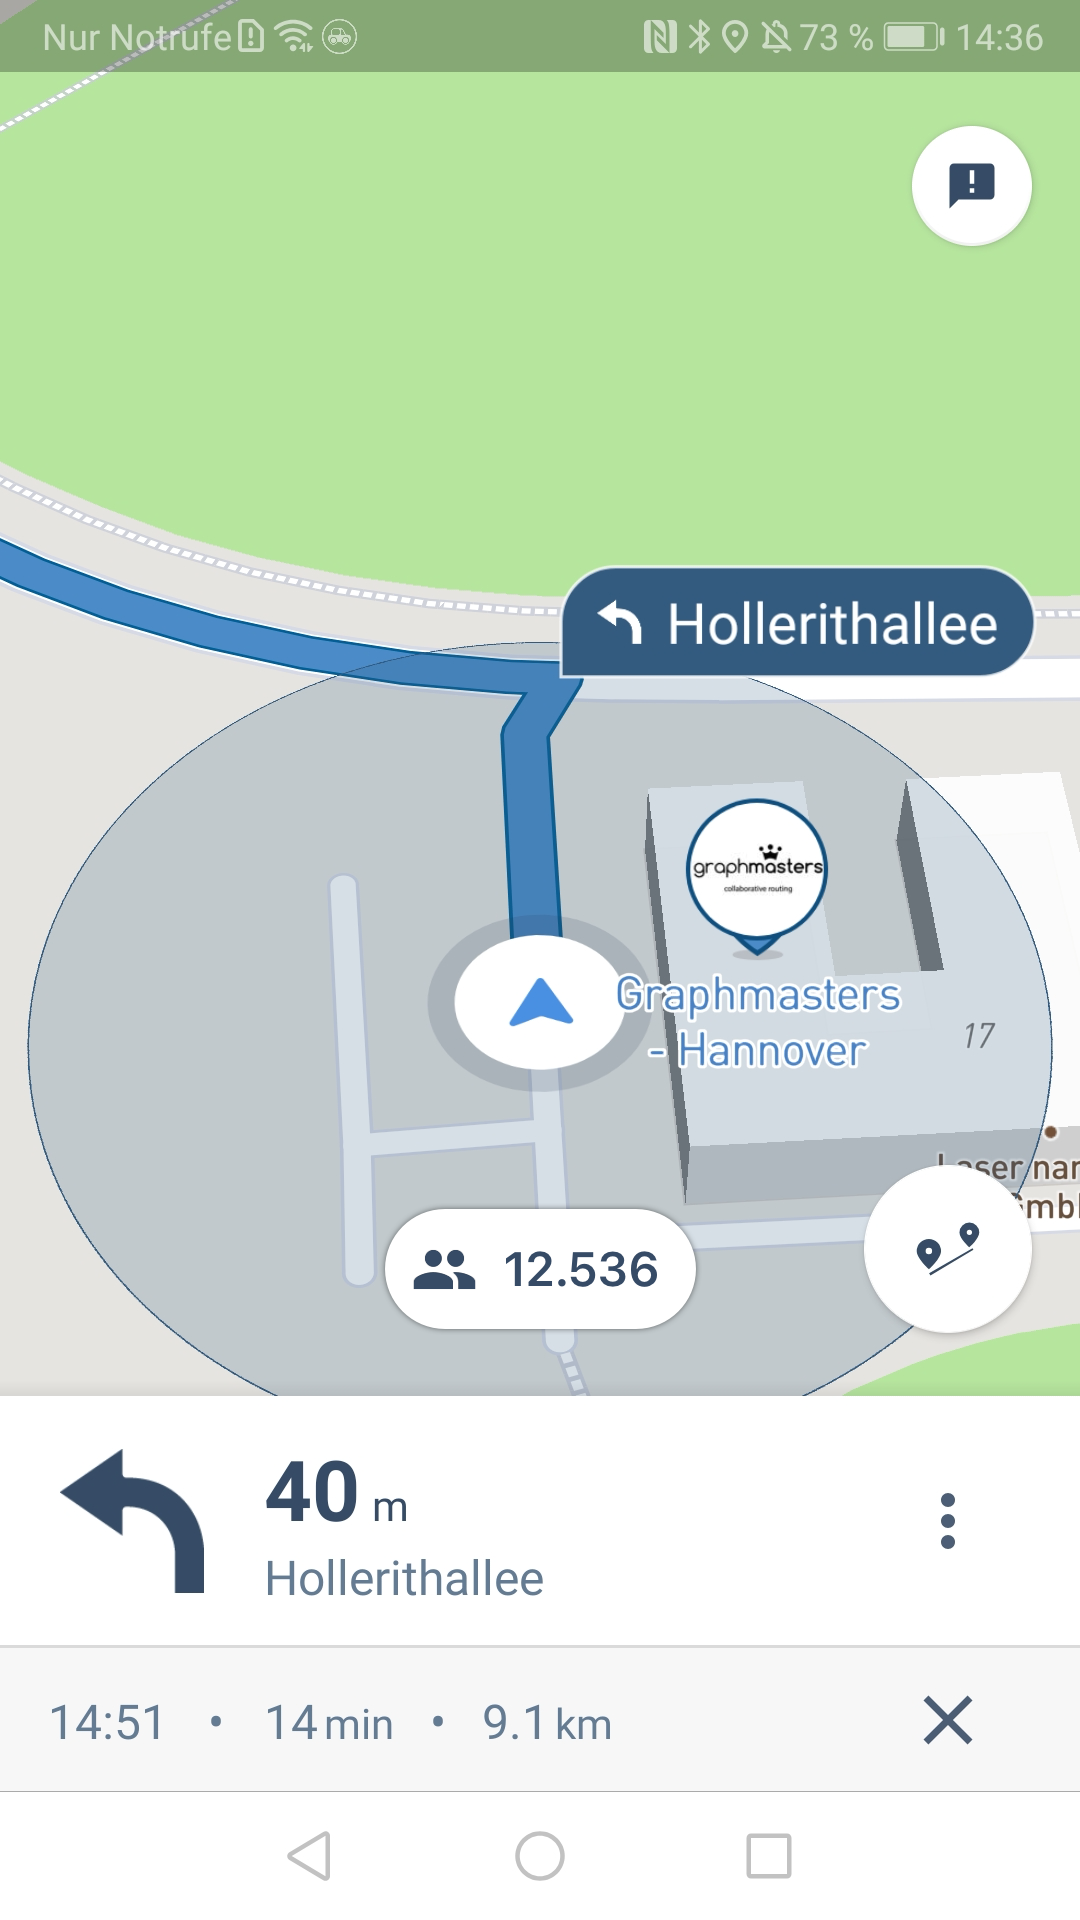
\includegraphics[width=.27\linewidth]{contents/06_model_evaluation/01_integration/res/01_collaborative_routing/prototype_1.png}
    }
    \hspace{.055\linewidth}
    \subfloat[Finales Design der Positionierung der Nutzerzahl]
    {
        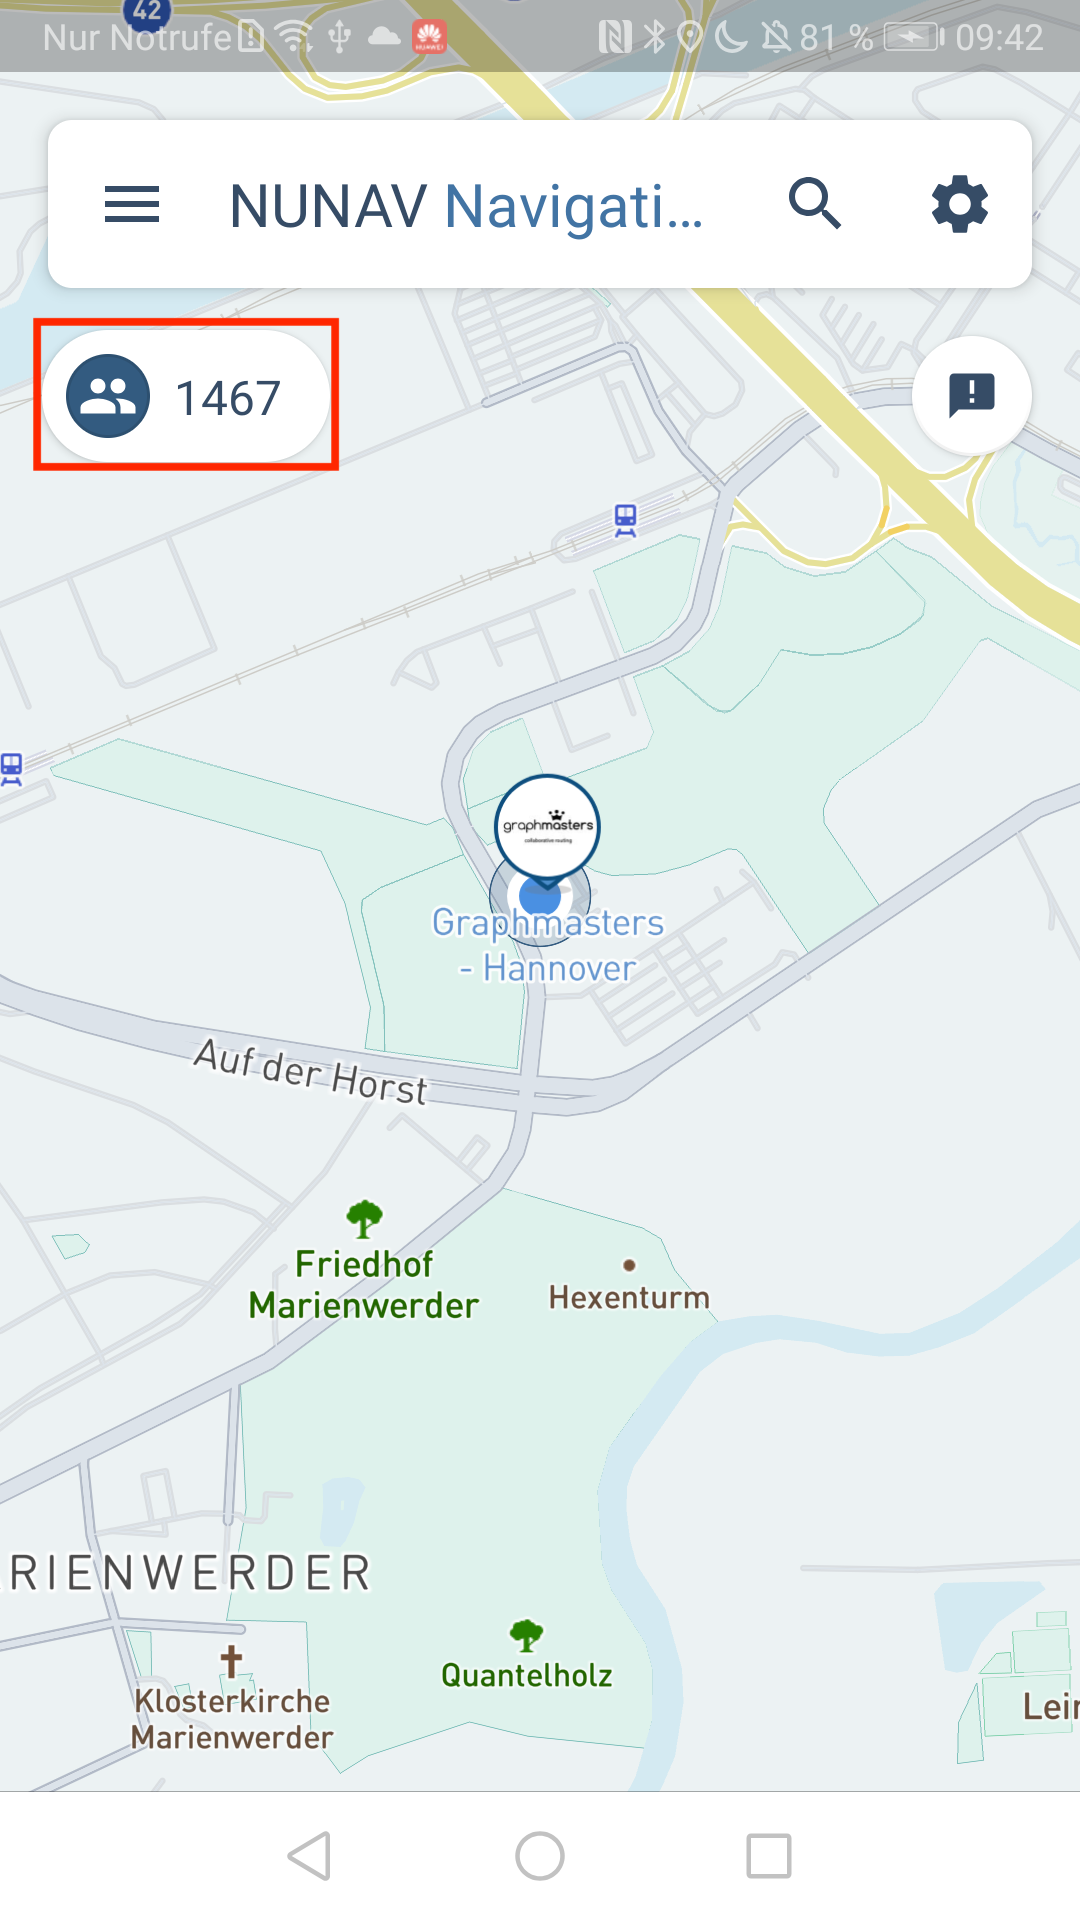
\includegraphics[width=.27\linewidth]{contents/06_model_evaluation/01_integration/res/01_collaborative_routing/final_1.png}
    }
    \hspace{.055\linewidth}
    \subfloat[Finales Design der kurzen Erklärung zum kollaborativen Routing]
    {
        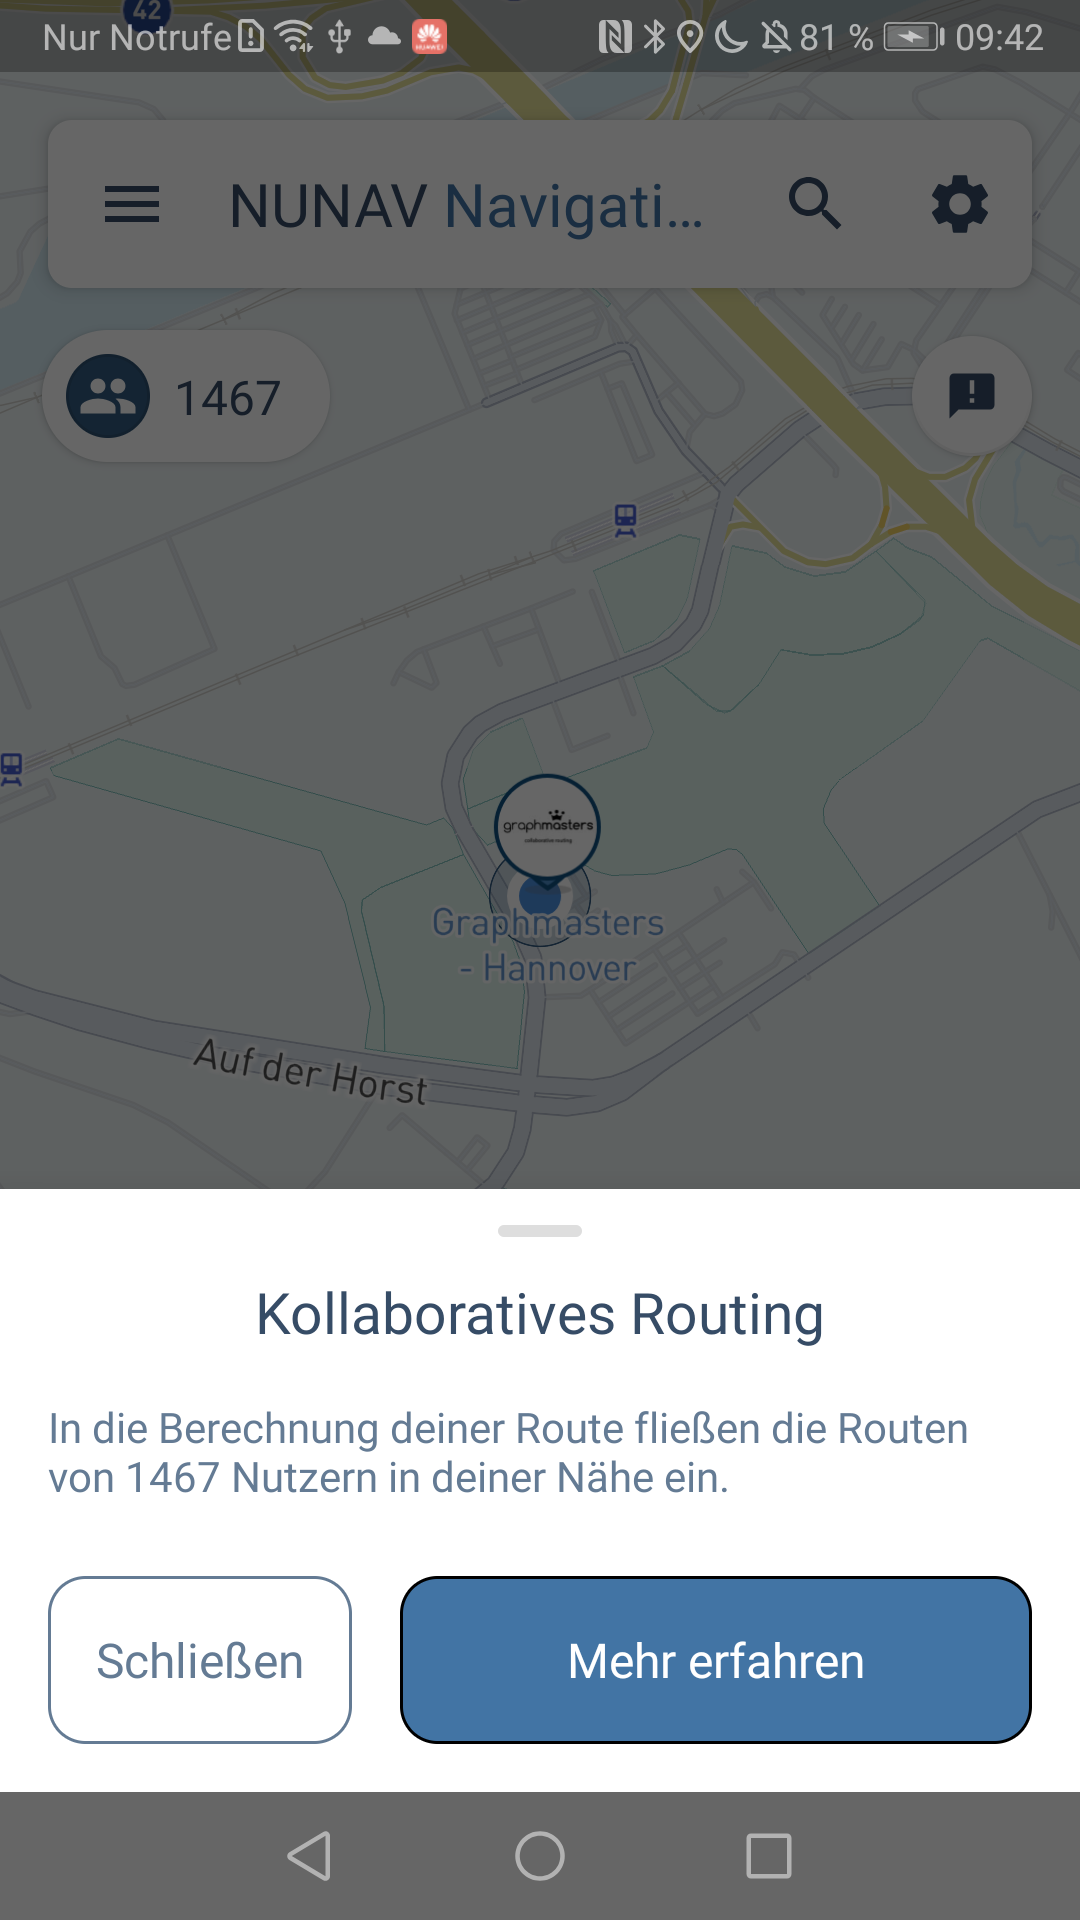
\includegraphics[width=.27\linewidth]{contents/06_model_evaluation/01_integration/res/01_collaborative_routing/final_2.png}
    }
    \caption{Prototyp und finale Designs für die Erklärung zum kollaborativem Routing}
    \label{fig:prototype_collaborative_routing}
\end{figure}